\chapter{Технологический раздел}

\section{Анализ систем управления базами данных}

Основными системами управления базами данных, работающими с реляционными базами данных являются PostgreSQL, Oracle Database и MySQL.

\begin{itemize}
	\item PostgreSQL --- СУБД, которая позволяет обеспечить полное соответствие требований ACID, создавать внешние ключи, триггеры, сложные процедуры и сложные команды SQL, бесплатно приобрести и получить поддержку СУБД.
	\item Oracle Database --- СУБД компании Oracle \cite{oracle}, которая обеспечивает высокую производительность, безопасность и масштабируемость.
	\item Служба базы данных MySQL --- управляемая служба базы данных, которая разрабатывается корпорацией Oracle \cite{mysql}. В возможности MySQL входят частичное соответствие требований ACID, обеспечение высокой скорости, поддержка большого числа функций.
\end{itemize}

\subsection{Выбор СУБД для решения задачи}

На основе приведенного описания систем управления базами данных можно выделить следующие критерии их сравнения:
\begin{itemize}
	\item K1 --- соответствие требованиям ACID;
	\item K2 --- бесплатное использование;
	\item K3 --- возможность создания триггеров.
\end{itemize}

Результаты сравнения СУБД приведены в таблице \ref{tab:dsm}.

\begin{table}[h]
    \caption{Сравнение СУБД}
    \begin{center}
        \begin{tabular}{|l|l|l|l|}
            \hline
            \textbf{СУБД} & \textbf{К1} & \textbf{К2} & \textbf{К3} \\ \hline
            PostgreSQL & + & + & + \\ \hline
            Oracle Database & - & - & + \\ \hline
            MySQL & - & + & + \\ \hline
        \end{tabular}
    \end{center}
    \label{tab:dsm}
\end{table}

По результатам сравнения можно сделать вывод о том, что для эффективного решения задачи следует использовать PostgreSQL, так как это СУБД с открытым исходным кодом, обеспечивающая соответствие свойствам ACID и создание триггеров.

\section{Средства реализации}

Исходя из требований, выдвинутых при проектировании системы, для реализации программного обеспечения в качестве основного языка программирования был выбран объектно-ориентированный и ориентированный на компоненты язык программирования C\# \cite{pl}.

Для разработки взаимодействия с базой данных был выбран фреймворк Entity Framework Core \cite{core}, который используется при программировании на языке C\# и позволяет работать с выбранной СУБД PostgreSQL.

В качестве среды разработки была выбрана Visual Studio \cite{vs}, которая автоматизирует процесс сборки приложений и имеет встроенную поддержку веб-приложений.

Для реализации уровня представления использовался фреймворк Blazor \cite{blazor}, позволяющий создавать пользовательский интерфейс, используя только язык программирования C\#.

\section{Детали реализации}

\subsection{Триггеры базы данных}

На листинге \ref{lst:delete_user_trigger.sql} показана реализация триггера, выполняющегося перед удалением пользователя.

\includelisting
    {delete_user_trigger.sql}
    {DML-триггер BEFORE DELETE на таблице пользователей}

Реализация триггера, выполнение которого происходит перед удалением продажи, представлена на листинге \ref{lst:delete_sale_trigger.sql}.   

\includelisting
    {delete_sale_trigger.sql}
    {DML-триггер BEFORE DELETE на таблице продаж}    

\subsection{Роли базы данных}

Создание роли неавторизованного пользователя представлено на листинге \ref{lst:create_not_auth_role.sql}

\includelisting
    {create_not_auth_role.sql}
    {Создание роли неавторизованного пользователя}
    
На листинге \ref{lst:create_customer_role.sql} показано создание роли покупателя.

\includelisting
    {create_customer_role.sql}
    {Cоздание роли покупателя}

Создание роли поставщика представлено на листинге \ref{lst:create_supplier_role.sql}

\includelisting
    {create_supplier_role.sql}
    {Создание роли поставщика}
    
На листинге \ref{lst:create_admin_role.sql} показано создание роли администратора.

\includelisting
    {create_admin_role.sql}
    {DML-триггер BEFORE DELETE на таблице пользователей}

\subsection{Полученный результат}

Далее приведены некоторые страницы разработанной информационной системы: на рисунке \ref{img:rating} показана страница с рейтингом вин, доступная только для покупателя, на рисунке \ref{img:supplierWines} --- страница с винами поставщика, кнопками для их добавления, изменения и удаления, доступная только для поставщика, и страница управления правами поставщиков, доступная только для администратора (рисунок \ref{img:suppliers}).
    
\includeimage
    {rating}
    {f}
    {h}
    {1.0\textwidth}
    {Страница с рейтингом вин (для покупателя)}

\begin{figure}[H]
	\begin{center}
		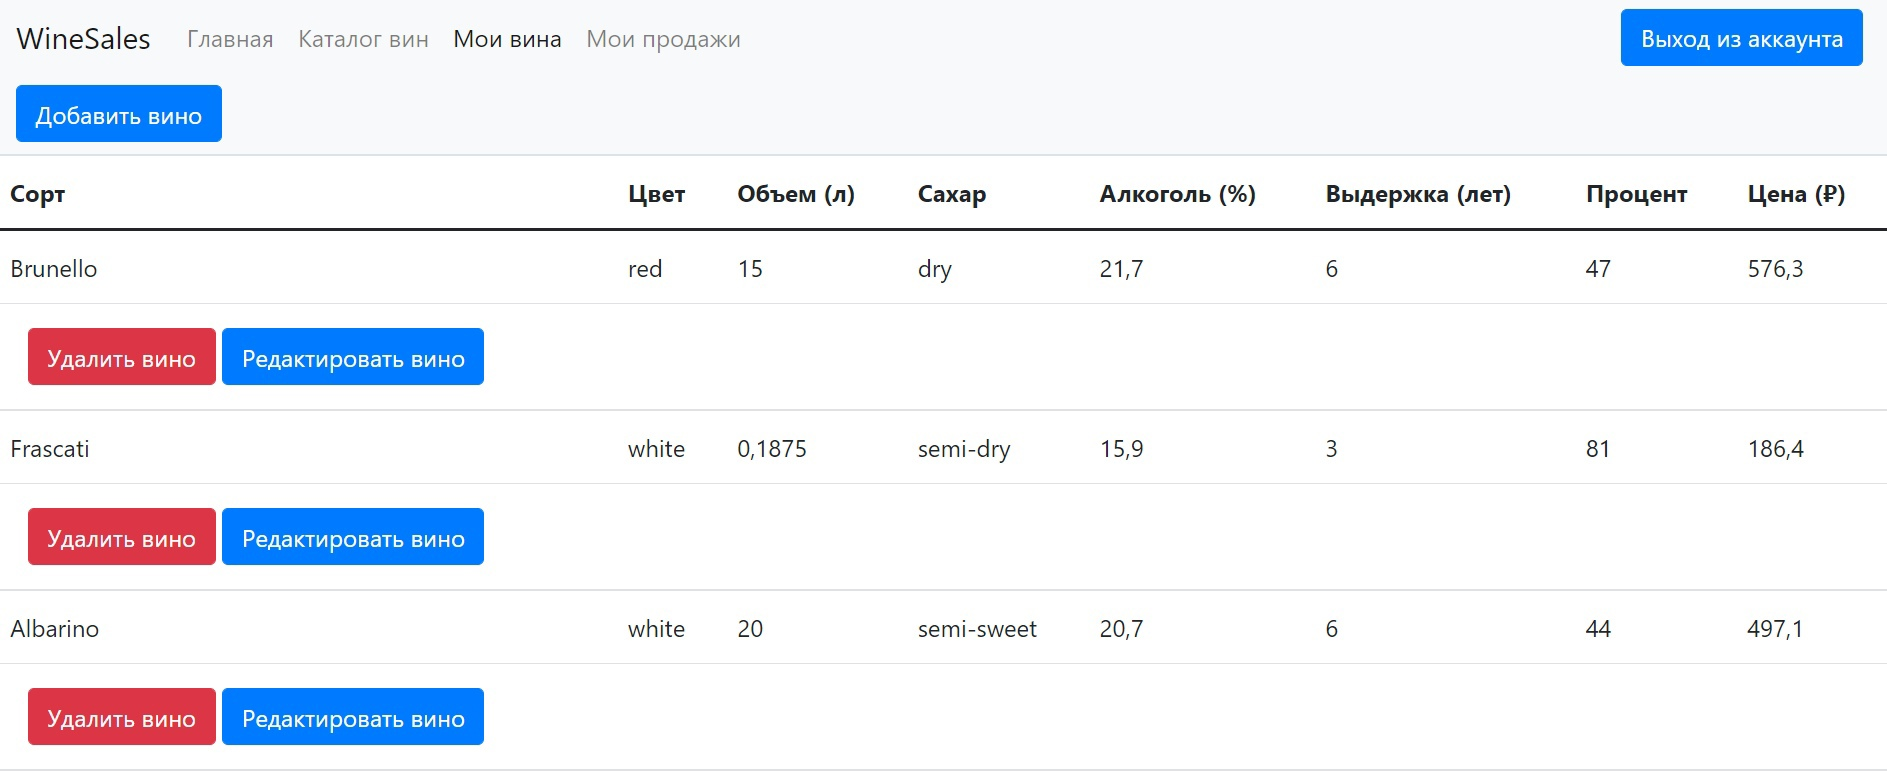
\includegraphics[scale=0.25]{inc/img/supplierWines.jpg}
	\end{center}
	\captionsetup{justification=centering}
	\caption{Страница с винами поставщика (для поставщика)}
	\label{img:supplierWines}
\end{figure}
    
\begin{figure}[H]
	\begin{center}
		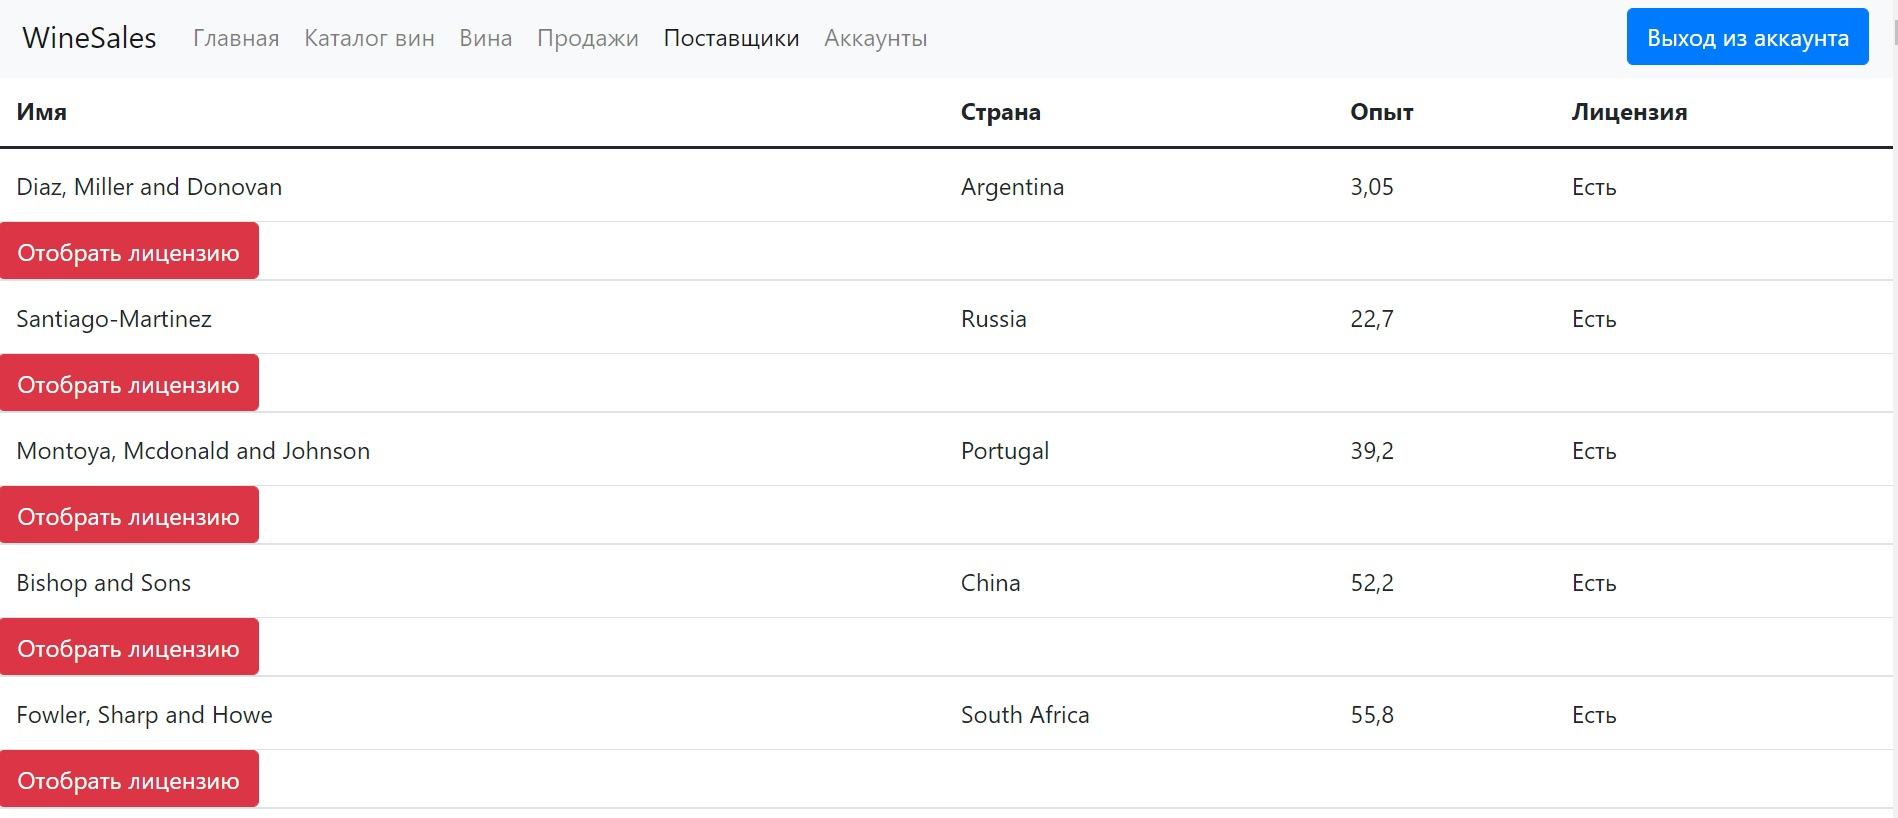
\includegraphics[scale=0.25]{inc/img/suppliers.jpg}
	\end{center}
	\captionsetup{justification=centering}
	\caption{Страница управления правами поставщиков (для администратора)}
	\label{img:suppliers}
\end{figure}
    
\section*{Вывод}

В данном разделе был проведен анализ систем управления базами данных, в результате которого была выбрана СУБД PostgreSQL. Также были описаны средства реализации, приведены детали реализации и представлен полученный результат.